\documentclass[12pt]{letter}

\usepackage{amsmath,amssymb}
\usepackage{nopageno}
\usepackage{enumitem}
\usepackage[a4paper, total={7.5in, 11.25in}]{geometry}
\usepackage{tikz}
\usepackage{pgfplots}
\pgfplotsset{compat=1.18}

\usetikzlibrary{calc,3d,decorations.pathmorphing,decorations.pathreplacing,decorations.markings,snakes,arrows.meta,patterns}
\tikzset{snake it/.style={decorate, decoration=snake}}

\begin{document}

Name: \hrulefill \quad Neptun code: \hrulefill

\begin{center}
(KTXFI1EBNF) Physics I. Test~1 Solutions \\
May~11,~2026 
\end{center}

\bigskip

\begin{enumerate}
\setcounter{enumi}{0}

\item  At what distance from Pluto does a Pluto-stationary satellite orbit in the plane of the equator if it remains constantly above the same point on Pluto's surface? ($M_{\mathrm{Pluto}}=1.305\cdot 10^{22}\,\mathrm{kg}$, \\ $T_{rot}=6.38723\,\mathrm{day}$, $R_{Pluto}=1188\,\mathrm{km}$, $G=6.6743\cdot 10^{-11}\,\mathrm{Nm^2/kg^2}$.)  

\begin{center}
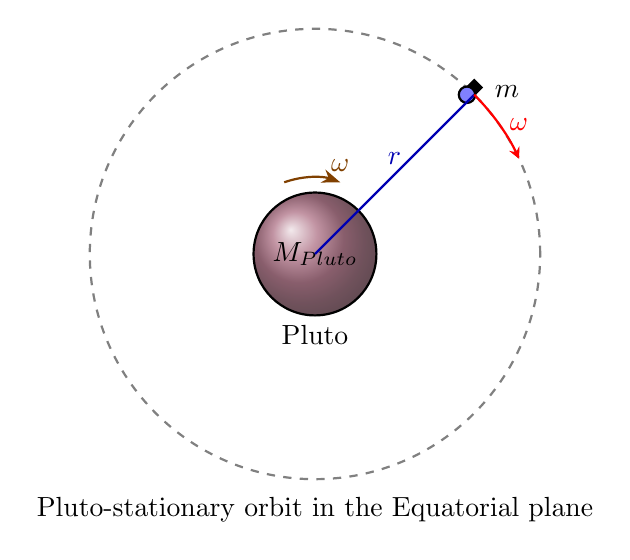
\begin{tikzpicture}[scale=1.3,>=Stealth,thick]
    % Mars (at center)
    \shade[ball color=orange!60!blue, opacity=0.8] (0,0) circle (0.6);
    \draw[thick] (0,0) circle (0.6);
    \node at (0,0) {$M_{Pluto}$};
    \node[below] at (0,-0.6) {Pluto};

    % Areosynchronous orbit (dashed line)
    \draw[dashed, gray] (0,0) circle (2.2);

    % Satellite (m) on the orbit
    \begin{scope}[rotate=45]
        \draw[fill=black] (2.2,0) rectangle (2.3,0.1); % Solar panels
        \draw[fill=black] (2.1,0) rectangle (2.2,0.1);
        \draw[fill=blue!50] (2.15, 0.05) circle (0.08); % Satellite body
        \node[right=5pt] at (2.2, 0.05) {$m$};
        
        % Radius (r) indication
        \draw[-, >=stealth, thick, blue!70!black] (0,0) -- (2.2,0) node[midway, above, sloped] {$r$};
        
        % Angular velocity direction
        \draw[->, >=stealth, thick, red] (2.2,0.0) arc[start angle=0, end angle=-20, radius=2.2] node[midway, right] {$\omega$};
    \end{scope}

    % Rotation of Pluto
    \draw[->, thick, orange!50!black] (-0.3,0.7) arc[start angle=110, end angle=70, radius=0.8] node[above] {$\omega$};

    % Caption
    \node at (0,-2.5) {Pluto-stationary orbit in the Equatorial plane};
\end{tikzpicture}
\end{center}

For a stationary orbit, the orbital period of the satellite must be equal to the rotation period of Pluto:
$$T = 6.38723\,\mathrm{days}.$$

Converting this into seconds:
$$T=6.38723 \cdot 24 \cdot 3600\,s\approx 5.51857\cdot 10^{5}\,\mathrm{s}.$$

The gravitational force provides the centripetal force:
$$\frac{GM_ {Pluto}m}{r^2}=m\frac{4\pi^2r}{T^2}.$$

After simplifying and solving for the orbital radius:
$$r=\sqrt[3]{\frac{GM_{Pluto}T^2}{4\pi^2}}.$$

Substituting the data:
$$r=\sqrt[3]{\frac{(6.6743\cdot 10^{-11}\,Nm^{2}/kg^{2})(1.305\cdot 10^{22}\,kg)(5.51857\cdot 10^{5}\,s)^2}{4\pi^2}}.$$

$$r\approx1.88\cdot 10^{7}\,\mathrm{m}.$$

Therefore, the 
$$r \approx 1.88\cdot 10^{4}\,\mathrm{km}$$
from the center of Pluto.

Since the radius of Pluto is approximately
$$R_{\mathrm{Pluto}}\approx1188\,\mathrm{km},$$
the altitude above the surface is
$$h=r-R_{\mathrm{Pluto}}\approx1.88\cdot 10^{4}-1.19\cdot 10^{3}.$$

$$\boxed{h \approx 1.76\cdot 10^{4}\,\mathrm{km}}$$

\hfill (10~points)

% ------------------------------------------------------------------------------------------------------------------------------------

\pagebreak
\item A $5\,\mathrm{kg}$ object slides down a $4$-meter-high incline that makes an angle of $45^\circ$ with the horizontal. What is the speed of the object when it reaches the bottom of the incline if it starts from rest at the top and:
\begin{enumerate}
    \item there is no friction between the object and the incline?
    \item the coefficient of friction is $0.1$? 
    \end{enumerate}
($g=9.81\,\mathrm{m/s^{2}}$)

\begin{center}
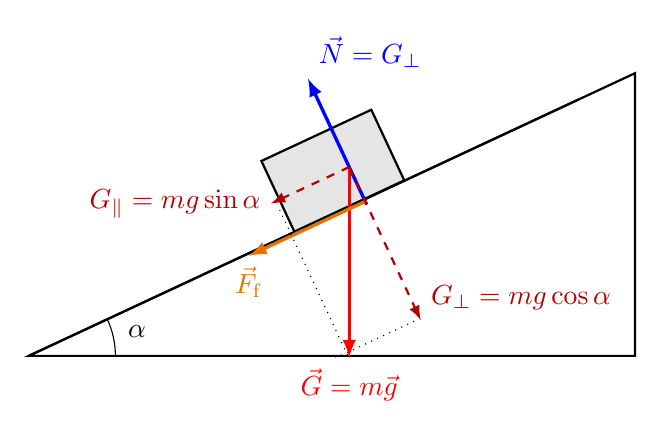
\begin{tikzpicture}[scale=1.1, >=latex]

% Parameters
\def\ang{25}
\def\L{7}
\def\H{2.8}

% Inclined plane
\draw[thick] (0,0) -- (\L,0) -- (\L,{\L*tan(\ang)}) -- cycle;
\draw[thick] (0,0) -- ({\L*cos(\ang)},{\L*sin(\ang)});

% Angle
\draw (1,0) arc[start angle=0,end angle=\ang,radius=1];
\node at (1.25,0.28) {$\alpha$};

% Block
\coordinate (O) at (3.7,1.73);
\begin{scope}[shift={(O)}, rotate=\ang]
  \draw[fill=gray!20, thick] (-0.7,0) rectangle (0.7,0.9);
  \coordinate (C) at (0,0.45);
\end{scope}

% Center of mass in global coordinates
\coordinate (G) at (3.7,2.18);

% Unit directions visually
% Forces
\draw[->, very thick, blue] (3.9,1.75) -- ++({90+\ang}:1.6)
  node[above right] {$\vec N=G_{\perp}$};

\draw[->, very thick, red] (G) -- ++(270:2.2)
  node[below] {$\vec G=m\vec g$};

\draw[->, very thick, orange!90!black] (3.9,1.79) -- ++({180+\ang}:1.5)
  node[below] {$\vec F_{\mathrm{f}}$};

% Components of weight
\draw[->, thick, red!70!black, dashed] (G) -- ++({270+\ang}:1.95)
  node[above right] {$G_{\perp}=mg\cos\alpha$};

\draw[->, thick, red!70!black, dashed] (G) -- ++({180+\ang}:1.0)
  node[left] {$G_{\parallel}=mg\sin\alpha$};

% Helper right triangle for decomposition
\draw[dotted] 
  ($(4.45,0.4)+({270+\ang}:0)$) -- 
  ($(4.45,0.4)+({180+\ang}:1.0)$);

\draw[dotted] 
  ($(2.2,3.18)+({270+\ang}:3.5)$) -- 
  ($(2.2,3.18)+({270+\ang}:1.65)$);
  
%\draw[dotted] 
%  ($(G)+({270+\ang}:1.75)$) -- 
%  ($(G)+({180+\ang}:1.25)$);


% Local axes
%\draw[->, thin] (5.6,2.7) -- ++({\ang}:1.0) node[right] {$x$};
%\draw[->, thin] (5.6,2.7) -- ++({90+\ang}:0.8) node[above] {$y$};

% Labels on plane
%\node at (4.8,1.25) [rotate=\ang] {slide};

\end{tikzpicture}
\end{center}


The height of the incline is
$$ h=4\,\mathrm{m}.$$

\begin{enumerate}
\item Without friction, mechanical energy is conserved:
$$mgh=\frac12 mv^2.$$

Therefore,
$$v=\sqrt{2gh}.$$

Substitution gives
$$v=\sqrt{2\cdot 9.81\,m/s^2\cdot 4\,m}\approx \boxed{8.9\,\mathrm{m/s}.}$$

\item With friction, the friction force is
$$F_f=\mu mg\cos\alpha.$$

The length of the incline is
$$s=\frac{h}{\sin\alpha}.$$

The work done by friction is
$$W_f=F_f s=\mu mg\cos\alpha \frac{h}{\sin\alpha}=\mu mgh\cot\alpha.$$

Using energy conservation with energy loss:
$$mgh-\mu mgh\cot\alpha=\frac12 mv^2.$$

Thus,
$$v=\sqrt{2gh(1-\mu\cot\alpha)}.$$

For
$$\alpha=45^\circ,\qquad \cot45^\circ=1,$$
we get
$$v=\sqrt{2gh(1-\mu)}.$$

Substitution:
$$v=\sqrt{2\cdot 9.81\,\mathrm{m/s^2}\cdot 4\,\mathrm{m}\cdot (1-0.1)}\approx\boxed{ 8.4\,\mathrm{m/s}}.$$

\end{enumerate}
\hfill (10~points)

% ------------------------------------------------------------------------------------------------------------------------------------

\pagebreak
\item At a temperature of $30{}^{\circ}\mathrm{C}$, a steel shaft with a diameter of $11.30\,\mathrm{cm}$ needs to be fitted with an aluminum ring with an inner diameter of $11.27\,\mathrm{cm}$ at the same temperature. The linear thermal expansion coefficient of steel is $12 \cdot 10^{-6}\,\mathrm{K}^{-1}$, and the linear thermal expansion coefficient of aluminum is $28.7 \cdot 10^{-6}\,\mathrm{K}^{-1}$. What temperature must the ring be heated to?

\bigskip
\begin{center}
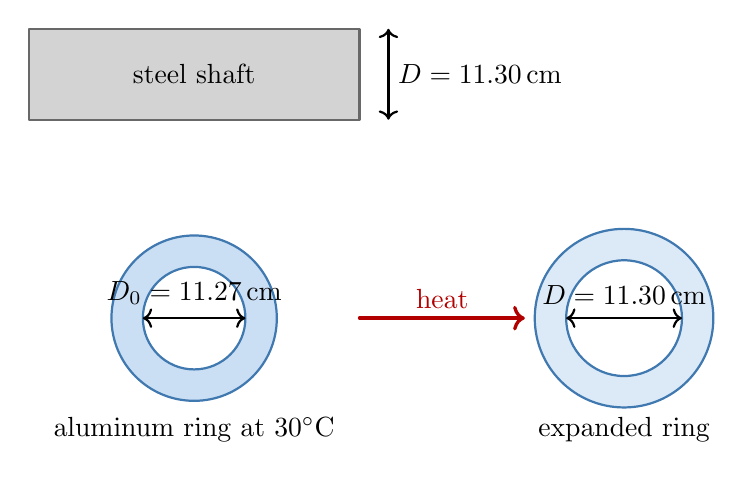
\begin{tikzpicture}[scale=1.05, line cap=round, line join=round]

% Colors
\definecolor{steel}{RGB}{130,130,130}
\definecolor{alum}{RGB}{80,150,220}

% Steel shaft
\fill[steel!35] (-2,0) rectangle (2,1.1);
\draw[thick, steel!80!black] (-2,0) rectangle (2,1.1);
\node at (0,0.55) {steel shaft};

% Shaft diameter arrow
\draw[<->, thick] (2.35,0) -- (2.35,1.1);
\node[right] at (2.35,0.55) {$D = 11.30\,\mathrm{cm}$};

% Aluminum ring, cold
\begin{scope}[xshift=0cm,yshift=-2.4cm]
  \fill[alum!30, even odd rule] (0,0) circle (1.0) (0,0) circle (0.62);
  \draw[thick, alum!80!black] (0,0) circle (1.0);
  \draw[thick, alum!80!black] (0,0) circle (0.62);
  \node at (0,-1.35) {aluminum ring at $30^\circ\mathrm{C}$};

  % Inner diameter arrow
  \draw[<->, thick] (-0.62,0) -- (0.62,0);
  \node[above] at (0,0.05) {$D_{0}=11.27\,\mathrm{cm}$};
\end{scope}

% Heating arrow
\draw[->, very thick, red!70!black] (2.0,-2.4) -- (4.0,-2.4);
\node[above, red!70!black] at (3.0,-2.4) {heat};

% Aluminum ring, expanded
\begin{scope}[xshift=5.2cm,yshift=-2.4cm]
  \fill[alum!20, even odd rule] (0,0) circle (1.08) (0,0) circle (0.70);
  \draw[thick, alum!80!black] (0,0) circle (1.08);
  \draw[thick, alum!80!black] (0,0) circle (0.70);
  \node at (0,-1.35) {expanded ring};

  \draw[<->, thick] (-0.70,0) -- (0.70,0);
  \node[above] at (0,0.05) {$D=11.30\,\mathrm{cm}$};
\end{scope}

\end{tikzpicture}
\end{center}

The aluminum ring must expand from
$$D_0=11.27\,\mathrm{cm}=0.1127\,\mathrm{m}$$
to
$$D=11.30\,\mathrm{cm}=0.113\,\mathrm{m}.$$

The linear thermal expansion formula is
$$D=D_0(1+\alpha\Delta T).$$

Thus,
$$\Delta T=\frac{D-D_0}{\alpha D_0}.$$

Substitution gives
$$\Delta T=\frac{0.113\,\mathrm{m}-0.1127\,\mathrm{m}}{(2.87\cdot 10^{-5}\,\mathrm{1/K})\cdot 0.1127\,\mathrm{m}}\approx 92.75\,\mathrm{K}.$$

The initial temperature is
$$T_0=30^\circ\mathrm{C}.$$

Therefore,
$$T=T_0+\Delta T=30^\circ\mathrm{C}+92.75^\circ\mathrm{C}\approx \boxed{122.75^\circ\mathrm{C}.}$$

\hfill (10~points)

% ------------------------------------------------------------------------------------------------------------------------------------

\pagebreak
\item A weather balloon floating at an altitude of several kilometers has a volume of $1800\,\mathrm{m}^{3}$. The temperature and pressure of the helium inside it are the same as those of the surroundings: $-50{}^{\circ}\mathrm{C}$ and $7 \cdot 10^{3}\,\mathrm{Pa}$, respectively.
\begin{enumerate}
\item How many moles of helium are in the balloon?
\item What is the mass of the helium gas? $\left(M = 4\,\frac{\mathrm{g}}{\mathrm{mol}}\right)$
\item What was the volume of the balloon when it was launched from Earth, if the gas inside the balloon was characterized by a temperature of $0{}^{\circ}\mathrm{C}$ and a pressure of $10^{5}\,\mathrm{Pa}$?
\end{enumerate}
($R=8.31\,\mathrm{J/K}$) 

\begin{center}
  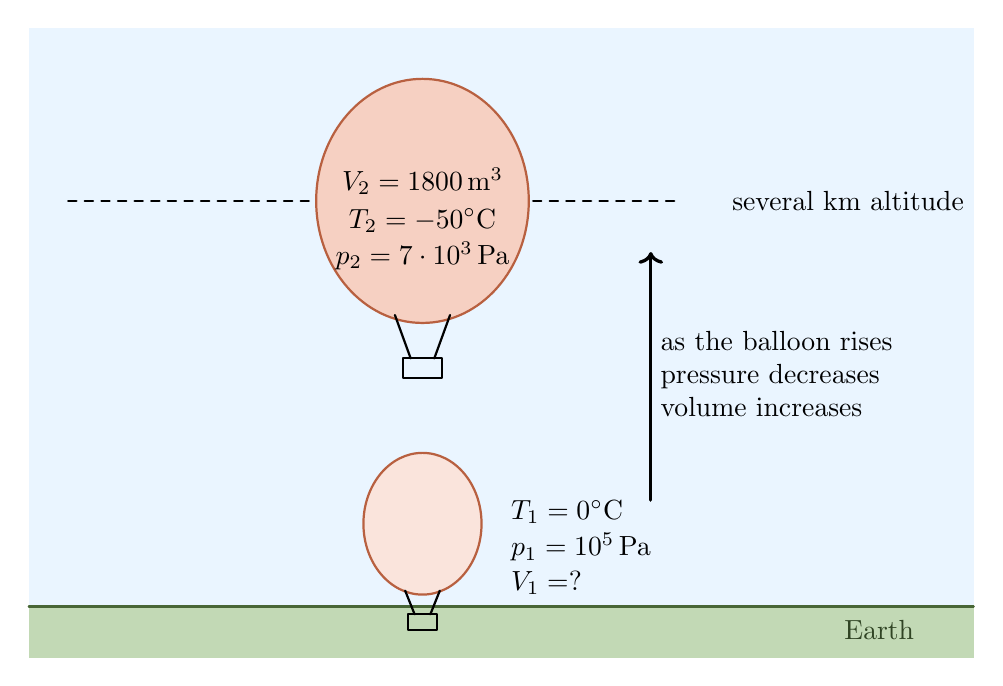
\begin{tikzpicture}[scale=1.0, line cap=round, line join=round]

% Colors
\definecolor{skyblue}{RGB}{170,215,255}
\definecolor{balloon}{RGB}{230,120,80}
\definecolor{earth}{RGB}{120,170,90}

% Background
\fill[skyblue!25] (-4,-2.8) rectangle (8,5.2);

% Earth / ground
\fill[earth!45] (-4,-2.8) rectangle (8,-2.15);
\draw[thick, earth!60!black] (-4,-2.15) -- (8,-2.15);
\node[earth!40!black] at (6.8,-2.45) {Earth};

% Altitude dashed line
\draw[dashed, thick] (-3.5,3.0) -- (4.25,3.0);
\node[left] at (8.0,3.0) {several km altitude};

% Balloon in the sky
\begin{scope}[shift={(1.0,3.0)}]
  \fill[balloon!35] (0,0) ellipse (1.35 and 1.55);
  \draw[thick, balloon!80!black] (0,0) ellipse (1.35 and 1.55);
  \draw[thick] (-0.35,-1.45) -- (-0.15,-2.0);
  \draw[thick] (0.35,-1.45) -- (0.15,-2.0);
  \draw[thick] (-0.25,-2.0) rectangle (0.25,-2.25);
  \node at (0,0.25) {$V_2=1800\,\mathrm{m^3}$};
  \node at (0,-0.25) {$T_2=-50^\circ\mathrm{C}$};
  \node at (0,-0.70) {$p_2=7\cdot10^3\,\mathrm{Pa}$};
\end{scope}

% Balloon at launch
\begin{scope}[shift={(1.0,-1.1)}]
  \fill[balloon!20] (0,0) ellipse (0.75 and 0.90);
  \draw[thick, balloon!80!black] (0,0) ellipse (0.75 and 0.90);
  \draw[thick] (-0.22,-0.85) -- (-0.10,-1.15);
  \draw[thick] (0.22,-0.85) -- (0.10,-1.15);
  \draw[thick] (-0.18,-1.15) rectangle (0.18,-1.35);
  \node[right] at (1.0,0.15) {$T_1=0^\circ\mathrm{C}$};
  \node[right] at (1.0,-0.30) {$p_1=10^5\,\mathrm{Pa}$};
  \node[right] at (1.0,-0.75) {$V_1=?$};
\end{scope}

% Upward arrow
\draw[->, very thick] (3.9,-0.8) -- (3.9,2.35);
\node[right, align=left] at (3.9,0.8)
{as the balloon rises\\pressure decreases\\volume increases};
\end{tikzpicture}
\end{center}

Given:
$$V=1800\,\mathrm{m^3},\qquad p=7\cdot 10^3\,\mathrm{Pa},\qquad T=-50^\circ\mathrm{C}=223.15\,\mathrm{K}.$$

\begin{enumerate}
\item From the ideal gas law,
$$pV=nRT.$$

Thus,
$$n=\frac{pV}{RT}.$$

Substitution:
$$n=\frac{(7\cdot 10^3\,\mathrm{Pa})(1800\,\mathrm{m^{3}})}{8.314\,\mathrm{J/K}\cdot 223.15\,\mathrm{K}}\approx\boxed{6.8\cdot 10^3\,\mathrm{mol}}.$$

\item The molar mass of helium is
$$M=4\,\mathrm{g/mol}=0.004\,\mathrm{kg/mol}.$$

The mass is
$$m=nM=(6.79\cdot 10^3\,\mathrm{mol})(0.004\,\mathrm{kg/mol})\approx\boxed{27\,\mathrm{kg}}.$$

\item At launch:
$$T_0=0^\circ\mathrm{C}=273.15\,\mathrm{K},\qquad p_0=10^5\,\mathrm{Pa}.$$

Using the same amount of gas:
$$\frac{pV}{T}=\frac{p_0V_0}{T_0}.$$

Thus,
$$V_0=\frac{pVT_0}{p_0T}.$$

Substitution:
$$V_0=\frac{pVT_0}{p_0T}=\frac{(7\cdot 10^3\,\mathrm{Pa})(1800\,\mathrm{m^{3}})(273.15\,\mathrm{K})}{(10^5\,\mathrm{Pa})(223.15\,\mathrm{K})}\approx\boxed{1.54\cdot 10^2\,\mathrm{m^3}}.$$

\end{enumerate}
\hfill (10~points)


% ------------------------------------------------------------------------------------------------------------------------------------

\pagebreak
\item An electron enters the region between the parallel plates shown in the figure halfway between the plates. The length of the plates is $l = 12\,\mathrm{cm}$, their separation is $d = 2\,\mathrm{cm}$, and the voltage between them is $U = 300\,\mathrm{V}$. What must the initial velocity of the electron be so that it just exits the region between the plates? ($m_{e}=9.1\cdot 10^{-31}\,\mathrm{kg}$, $e=1.6\cdot 10^{-19}\,C$) 

\begin{center}
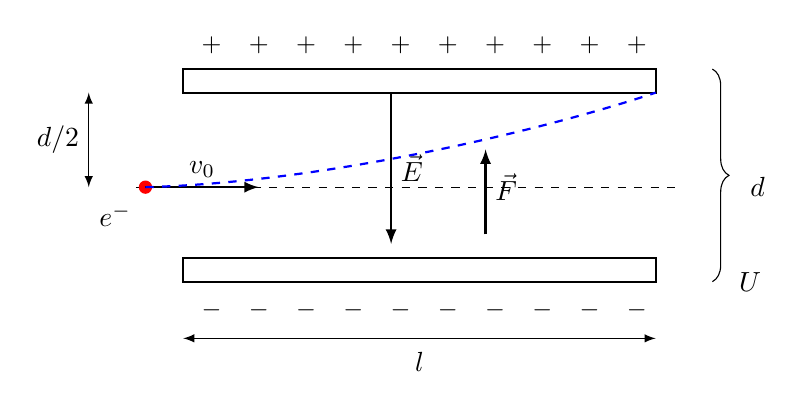
\begin{tikzpicture}[scale=1.2, >=latex]

% Parameters
\def\L{5}
\def\d{2}

% Plates
\draw[thick] (0,0) rectangle (\L,0.25);
\draw[thick] (0,-\d) rectangle (\L,-\d+0.25);

% Charges
\foreach \x in {0.3,0.8,...,4.8}
{
    \node at (\x,0.5) {\small $+$};
}

\foreach \x in {0.3,0.8,...,4.8}
{
    \node at (\x,-2.3) {\small $-$};
}

% Midline
\draw[dashed] (-0.5,-\d/2) -- (\L+0.2,-\d/2);

% Electron
\fill[red] (-0.4,-\d/2) circle (2pt);
\node[left] at (-0.45,-1.3) {$e^-$};

% Initial velocity
\draw[->, thick] (-0.4,-\d/2) -- (0.8,-\d/2);
\node[above] at (0.2,-\d/2) {$v_0$};

% Trajectory
\draw[thick, dashed, blue]
(-0.4,-\d/2)
.. controls (1.5,-0.95) and (3.8,-0.4)
.. (\L,0);

% Electric field
\draw[->, thick] (2.2,0.0) -- (2.2,-1.6);
\node[right] at (2.2,-0.8) {$\vec{E}$};

% Electric force
\draw[->, thick] (3.2,-1.5) -- (3.2,-0.6);
\node[right] at (3.2,-1.0) {$\vec{F}$};

% Length
\draw[<->] (0,-\d-0.6) -- (\L,-\d-0.6);
\node at (\L/2,-\d-0.85) {$l$};

% Separation
\draw[decorate, decoration={brace, amplitude=6pt, mirror}]
(\L+0.6,-\d) -- (\L+0.6,0.25);

\node[right] at (\L+0.9,-\d/2) {$d$};

% Voltage
\node at (\L+1.0,-\d/2-1.0) {$U$};

% Vertical displacement
\draw[<->] (-1.0,-\d/2) -- (-1.0,0);
\node[left] at (-1.0,-0.5) {$d/2$};

\end{tikzpicture}
\end{center}

Given:
$$l=12\,\mathrm{cm}=0.12\,\mathrm{m},\qquad d=2\,\mathrm{cm}=0.02\,\mathrm{m},\qquad U=300\,\mathrm{V}.$$

The electric field between the plates is
$$E=\frac{U}{d}.$$

Thus,
$$E=\frac{300}{0.02}=15000\,\mathrm{V/m}.$$

The electric force acting on the electron is
$$F=eE.$$

Therefore, the acceleration of the electron is
$$a=\frac{F}{m_e}=\frac{eE}{m_e}.$$

Substituting the values:
$$a=\frac{(1.602\cdot10^{-19}\,\mathrm{C})(15000\,\mathrm{V/m})}{9.109\cdot10^{-31}\,\mathrm{kg}}\approx   2.637\cdot10^{15}\,\mathrm{m/s^2}.$$

The electron enters halfway between the plates, therefore it must move vertically by
$$y=\frac{d}{2}=0.01\,\mathrm{m}$$
in order to just reach the upper plate at the exit.

The vertical motion is uniformly accelerated:
$$y=\frac{1}{2} at^2.$$

Thus,
$$0.01\,\mathrm{m}=\frac12(2.637\cdot10^{15}\mathrm{m/s^2})t^2.$$

Solving for the time:
$$t=\sqrt{\frac{2\cdot0.01\,\mathrm{m}}{2.637\cdot10^{15}\,\mathrm{m/s^2}}}\approx 2.754 \cdot10^{-9}\,\mathrm{s}.$$

The horizontal motion is uniform:
$$l=v_0 t.$$

Therefore,
$$v_0=\frac{l}{t}.$$

Substituting the values:
$$v_0=\frac{l}{t}=\frac{0.12\,\mathrm{m}}{2.754 \cdot10^{-9}}\,\mathrm{s}\approx 4.358\cdot 10^7\,\mathrm{m/s}.$$

Therefore, the required initial velocity is
$$\boxed{v_0\approx 4.36\cdot10^7\,\mathrm{m/s}}$$
\hfill (10~points)

\end{enumerate}

% ------------------------------------------------------------------------------------------------------------------------------------

Requirement for obtaining the course signature: achieving at least 40\% (20\,points) on the midterm exam.

Grades: 0--25 points: Fail (1), 26--30 points: Pass (2), 31--37 points: Satisfactory (3), 38--45 points:~Good~(4), 46--50 points: Excellent (5).

\rightline{Dr.~Gabor FACSKO}
\rightline{\textit{facsko.gabor@uni-obuda.hu}}

\vfill

\end{document}





